\documentclass{article}
\usepackage[utf8]{inputenc}

\title{A* Revisited}
\author{Rob Bishop and Daniel Power }
\date{December 2018}

\usepackage{natbib}
\usepackage{graphicx}
\usepackage{algorithm}
\usepackage{algorithmic}

\begin{document}

\maketitle

\section{Overview}
This report is designed to accompany and supplement the submitted application, which has been designed by us to emulate and improve on the A* algorithm as it was presented in class. Out additions to the assignment include a complete rewrite of the codebase from Javascript to C++, similar efficiency tricks as were employed in the submitted assignment to increase speed, as well as an implementation of Jump Point Search, which can drastically speed up times for specific map types.

\section{Problem: Flexibility and Performance}
This project managed to combine two of our favourite aspects of the semester: The fantastic SFML C++ library, as well as the A* pathfinding algorithm. After making numerous concessions to achieve the best speed we could in the assignment's Javascript environment, we decided that the speed of a compiled language and the flexibility of a visualization library like SFML would provide us with both adequate performance and challenge. Additionally, by using a binary application, we would be able to load arbitrary maps from disk dynamically, which would allow us to test in multiple environments quickly.

The A* pathfinding algorithm is said to be one of the most well known algorithms in computer science. First published in 1968\footnote{Hart, P. E.; Nilsson, N. J.; Raphael, B. (1968). "A Formal Basis for the Heuristic Determination of Minimum Cost Paths". } it is essentially the single-path version of Dijkstras algorithm with the addition of a heuristic function. Through it's use of an (admissible) heuristic, it is guaranteed to be optimal in that any similar search function can not explore fewer nodes than A*.

For our problem instance, we will be exploring the performance of our algorithm compared to the assignment paths, as well as some arbitrary environments.

\begin{figure}[h!]
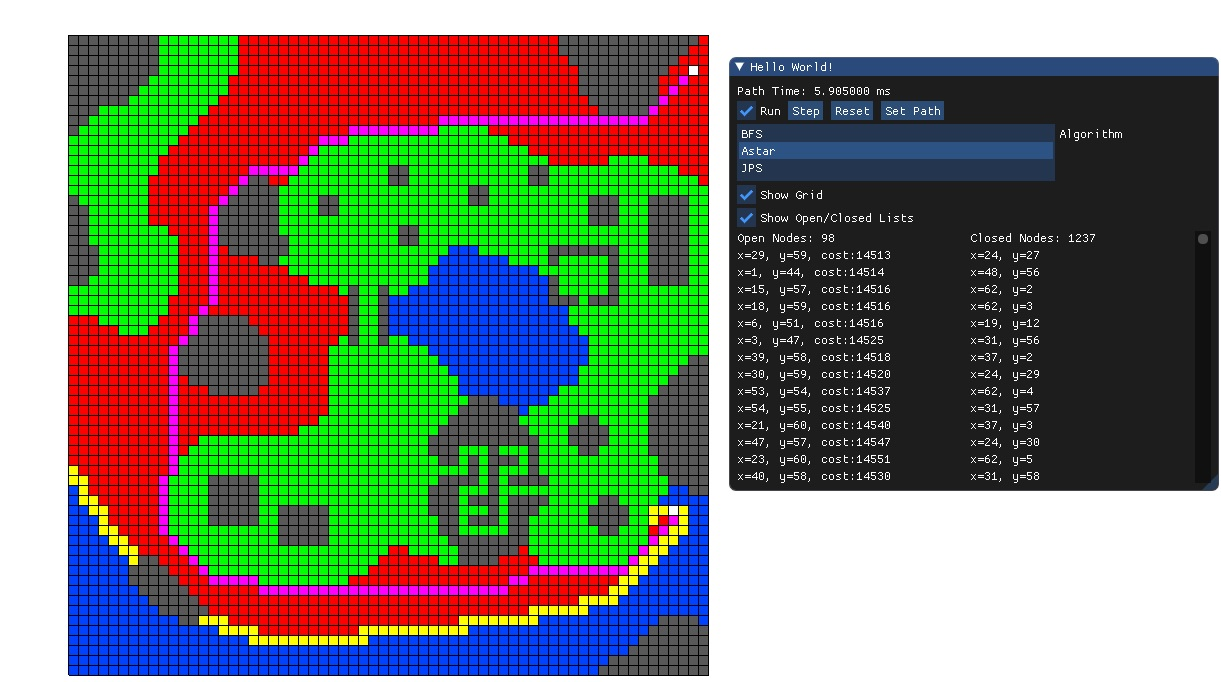
\includegraphics[width=\textwidth]{astar}
\caption{A screenshot of our application}
\end{figure}
\newpage
\section{Methodology}
The project can be broadly broken up into 3 steps:
\begin{itemize}
    \item Creating the GUI and visualization / loading of maps
    \item Implementing the A* algorithm
    \item Optimizing the A* algorithm
\end{itemize}
Though our initial intentions were that the first two would be trivial, in practice they proved to be more difficult than we expected. Discussion of the particulars of C++ and our implementation of the GUI are beyond the scope of this report, however.
\subsubsection*{The A* algorithm}
\begin{algorithm}
\caption{A* Search: basic version}
\begin{algorithmic}
\STATE initialize open list with first location
\STATE initialize an empty closed list
\FOR{infinity}
\IF{open list is Empty}
return failure
\ENDIF \\
\STATE current node = node in open list with lowest f score
\IF{current node is goal node}
return success: reconstruct path
\ENDIF
\IF{current node is in the closed list}
\STATE continue 
\ENDIF
\FOR{Each legal neighbour of current node}
\STATE let node N be a node constructed from the neighbour
\STATE let N's g-cost = the g-cost of current node + travel distance
\STATE let N's f-cost = the result of a heuristic $h(N)$
\STATE let N's parent = current node
\STATE add N to the open list
\ENDFOR
\ENDFOR
\STATE 
\end{algorithmic}
\end{algorithm}

While the A* algorithm is deceptively simple, the choice of data structures, looking conditions, heuristics and many other elements can have a massive impact on performance. We will discuss several optimizations in detail:
\begin{itemize}
    \item Caching the open list for $O(1)$ lookup
    \item using an efficient open list structure for min-retrieval
    \item Minimizing node size
\end{itemize}
\subsubsection*{Caching the Open List}
In order to prevent the open list from being overtaken by a large number of duplicates, it is nessecary to see if any of the legal neighbours of a node are already present on the open list. To this end, we elected to use an array of the same size as the problem space. By storing a node's G cost in the [x][y] location of this 2d array, we can see if our newly expanded node exists already with a lower score - meaning there is already a faster route to it. In such a case we can avoid creating a new node, avoid calculating and of it's scores, and save on both space and time.
\subsubsection*{Open list data structure}
Because A* requires repeated access to the lowest element, the ideal data structure for the open list is a priority queue. Much has been written about priority queues and their usefulness for the A* algorithm, including the creation of abstract and confounding data structures such as the Fibonacci Heap\footnote{Fredman, Michael Lawrence; Tarjan, Robert E. (July 1987). "Fibonacci heaps and their uses in improved network optimization algorithms" Journal of the Association for Computing Machinery.} or Brodal queues\footnote{Gerth Stølting Brodal (1996). Worst-case efficient priority queues. Proc. 7th ACM-SIAM Symposium on Discrete Algorithms}. For our implementation we have elected to use a binary min-heap as implemented by the C++ STL. This data structure provides $O(\log_n)$ retrieval of the minimum element.
\subsubsection*{Minimizing Node Size}
Despite best efforts to prune nodes, the open list will invariably contain many nodes, and minimizing their size is paramount to being able to work on larger maps. As such each element of a node must be carefully considered. As such, our pathfinding nodes contain very little actual data:
\begin{itemize}
    \item unsigned integer index
    \item unsigned integer sector
    \item unsigned integer g-score
    \item (A* only) unsigned integer f-score
\end{itemize}

\subsubsection*{Heuristics}
For our heuristic we elected to use primarily euclidean distance, however our algorithm has 4 as well as 8 directional Manhattan distance available. While euclidean distance, with it's expensive floating point operations, is undoubtedly slower, it is also the most accurate and as such the choice of heuristics is always one of inherent tradeoff.

\subsection*{Results \& Discussion}
We were able to consistently beat the times of our A* implementation from assignment 2 on several of the maps. In particular this time seems most significant on the smaller maps, which is likely a result of JIT compilation of various javascript functions.
\begin{figure}[h!]
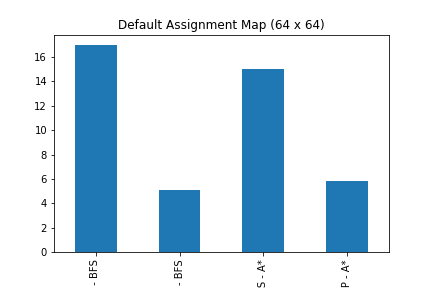
\includegraphics[width=\textwidth]{defaultMap}
\caption{Comparison of Javascript and CPP application times}
\end{figure}

All these tests were carried out on a desktop computer running the Windows 7 operating system, with an Intel i5 3.4Ghz processor and 16GB of DDR3 RAM.

\begin{figure}[h!]
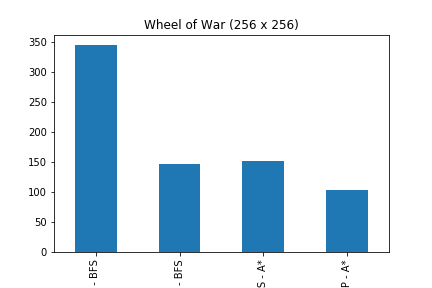
\includegraphics[width=\textwidth]{starcraft}
\caption{Comparison of Javascript and CPP application times}
\end{figure}

\begin{figure}[h!]
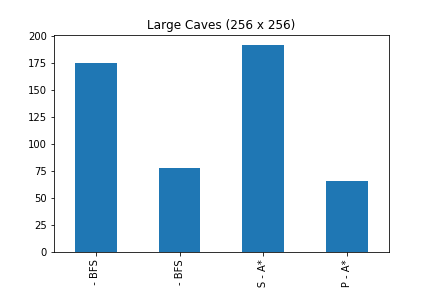
\includegraphics[width=\textwidth]{bigCaves}
\caption{Comparison of Javascript and CPP application times}
\end{figure}
\newpage

\section{Conclusion (AND JPS)}
In conclusion we are quite pleased with the performance of our C++ implementation of both the suite and the A* algorithm. In addition to being very performant, the code is written using many OOP features and laid out in a way that would make using it as a library on another project much easier to implement than a javascript application.

\subsection{JPS}
One of our ambitions was to implement Jump Point search, being excited for the performance gains it promises. While we have implemented JPS in our assignment, our current implementation is very inefficient. It offers time savings when used in open areas on larger maps, but in maps with tight corners and small areas performs worse than our vanilla A*. Nevertheless the logic is extremely promising, as the debug output shows just how few nodes are expanded using this technique.

\begin{figure}[h!]
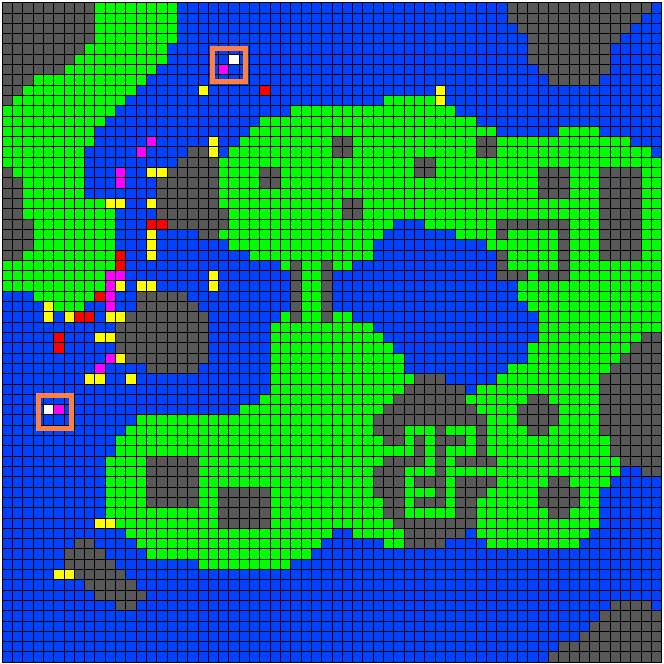
\includegraphics[width=\textwidth]{jps}
\caption{Jump Point search's open and closed node structure. The start and end points are accentuated by orange squares}
\end{figure}


% \bibliographystyle{plain}
% \bibliography{references}
\end{document}

% \begin{figure}[h!]
% \centering
% 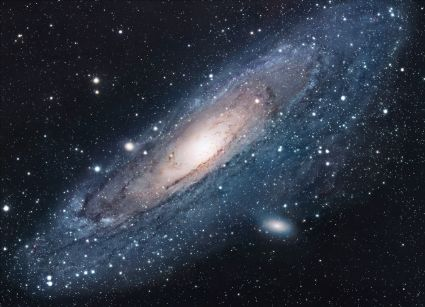
\includegraphics[scale=1.7]{universe}
% \caption{The Universe}
% \label{fig:universe}
% \end{figure}